%%\documentclass[journal,12pt,draftclsnofoot,onecolumn]{IEEEtran}
%%\documentclass[journal]{IEEEtran}
\documentclass[10pt,conference]{IEEEtran}

\usepackage{cite,comment,url}
\usepackage[dvips]{graphicx}
\usepackage{caption}
%\usepackage[caption=false,font=footnotesize]{subfig}
\usepackage{float}
\usepackage{enumerate}
\usepackage{epstopdf}

\usepackage{algorithmic}
\usepackage{algorithm}
\usepackage{multirow,subfig,epsfig}
\usepackage{amstext}

\newtheorem{mydef}{Definition}
\newtheorem{mytheo}{Theorem}

\usepackage{graphicx}
\usepackage{epstopdf}

\usepackage[namelimits]{amsmath}
\usepackage{amssymb}
\usepackage{cite}
\usepackage{array}
\usepackage{mdwmath}
\usepackage{mdwtab}

\usepackage{subfloat}

\usepackage{amsmath,amsthm}

\usepackage{booktabs}

\newtheorem{lem}{Lemma}
%%\usepackage{subcaption}

\setlength{\abovedisplayskip}{1mm}
\setlength{\belowdisplayskip}{1mm}
\IEEEoverridecommandlockouts

\begin{document}

%2 or two?
%
\title{
Analytical Optimal Solution of Selfish Node Detection with $2$-hop Constraints in OppNets: A Pontryagin's Maximum Principle Approach
}
\author{A, B, C\\
        School of Cyber Sci. \& Engr., Southeast University, Nanjing, China\\
        Key Lab of CNII, MOE, Southeast University, Nanjing, China\\
        Jiangsu Provincial Key Laboratory of Computer Network Technology, Southeast University, Nanjing, China\\
%        \{yanggao, juntao, zuyan94\}@seu.edu.cn
        }
\maketitle

\begin{abstract}
Selfish detection in the opportunistic networks offers an effective means
to mitigate the routing performance degradation,
but faces many challenges from the balance between 
the cost and the effect of detection behaviors.
%Blackhole detection in the opportunistic networks
%offers an effective means
%to mitigate the routing performance degradation,
%but faces many challenges from corrupted nodes
%due to their collusion behaviors.
%Most existing effort in the literature focuses on
%the blackhole feature extraction from the message exchange.
%However, the decay effect of features
%and the forged features from the corrupted node,
%which acts as the rational node in performing message exchange,
%degrade the performance of the detection.
%In this paper, we investigate the evidence construction,
%i.e., the direct and indirect evidence with the statistical parameters
%in message exchange.
%Specifically, we construct behavior classifiers
%to distinguish the blackhole behaviors from rational ones
%and design the collusion filtering strategy
%to improve the detection accuracy by
%separating corrupted nodes from rational ones, respectively,
%laying a behavior identification foundation.
%The Contact Evidence-driven Blackhole Detection
%based on machine learning (CEBD)
%is proposed to improve the routing performance.
%The soundness of the proposed scheme is verified statistically
%and the detection accuracy is evaluated
%based on RWP trace and Shanghai taxi trace.
%Extensive simulations show that
%our scheme outperforms
%the benchmarks, including SDBG, Li and MDS,
%in terms of the delivery ratio in various scenarios.
\end{abstract}


%\begin{abstract}
Selfish detection in the opportunistic networks offers an effective means
to mitigate the routing performance degradation,
but faces many challenges from the balance between 
the cost and the effect of detection behaviors.
%Blackhole detection in the opportunistic networks
%offers an effective means
%to mitigate the routing performance degradation,
%but faces many challenges from corrupted nodes
%due to their collusion behaviors.
%Most existing effort in the literature focuses on
%the blackhole feature extraction from the message exchange.
%However, the decay effect of features
%and the forged features from the corrupted node,
%which acts as the rational node in performing message exchange,
%degrade the performance of the detection.
%In this paper, we investigate the evidence construction,
%i.e., the direct and indirect evidence with the statistical parameters
%in message exchange.
%Specifically, we construct behavior classifiers
%to distinguish the blackhole behaviors from rational ones
%and design the collusion filtering strategy
%to improve the detection accuracy by
%separating corrupted nodes from rational ones, respectively,
%laying a behavior identification foundation.
%The Contact Evidence-driven Blackhole Detection
%based on machine learning (CEBD)
%is proposed to improve the routing performance.
%The soundness of the proposed scheme is verified statistically
%and the detection accuracy is evaluated
%based on RWP trace and Shanghai taxi trace.
%Extensive simulations show that
%our scheme outperforms
%the benchmarks, including SDBG, Li and MDS,
%in terms of the delivery ratio in various scenarios.
\end{abstract}

\begin{IEEEkeywords}
OppNet, Selfish, Black (Gray) Hole, ODE, Pontryagin's maximal principle
\end{IEEEkeywords}
%\IEEEpeerreviewmaketitle

\section{Introduction}
\label{sec:intro}
Exploiting mobile nodes to transmit message in
opportunistic networks(OppNets) has been attracting
increasing research attentions
\cite{DBLP:conf/sigcomm/SouzaMSMCC16,
DBLP:conf/infocom/LuSP16,
DBLP:conf/mobicom/RadenkovicH17,
DBLP:conf/infocom/SakaiSK19,
DBLP:journals/comsur/JedariXN18,
DBLP:journals/tmc/LoretiB20}.
With a widespread use and availability of
mobile communication devices, numerous applications
emerge based on message transmission in OppNets, especially 
in mobile social networks (OMSNs).
Opportunistic computing utilize the shared resources
in  OMSNs to provide a platform for the execution of
distributed computing tasks,

The main contributions are as follows:

\begin{itemize}
\item {we formulate the ordinary differential equation model (ODE)
to capture and analytically evaluate the state transition of nodes
in OppNets without detection and with complete detection.}
\item {we propose an optimal solution of selfish node detection
based on the Pontryagin's maximum principle
to achieve the tradeoff between the detection cost
and the reward of selfish behaviors.}
\item {we conduct experiments to evaluate
the effectiveness of the proposed model
and the optimal selfish detection solution 
in terms of the total cost, the wasted reward and the node state transition.}
\end{itemize}

The rest of this paper is organized as follows.
The literature is reviewed in Section~\ref{sec:related}.
We formulate the problem in Section~\ref{sec:preli}.
The change of network state without detection and with fully detection
is investigated in Section~\ref{sec:ode_model}.
The optimal solution of the selfish detection in OppNets
is presented in Section~\ref{sec:opt_detect},
and evaluated in Section~\ref{sec:pe}.
The paper concludes in Section~\ref{sec:conclude}.

\section{Related Work}
\label{sec:related}
\subsection{Message Transmission in Selfish OppNets}
%~\cite{DBLP:journals/tmc/ChoiSLW12}��
%~\cite{DBLP:journals/tmc/Hernandez-Orallo15}��
%~\cite{DBLP:conf/icdcs/GaoMAH18}
%~\cite{DBLP:journals/fgcs/JedariXCDTA19}
%~\cite{DBLP:journals/tvt/NomikosCVWK20}
%~\cite{DBLP:journals/tie/DiasRXM15}
%~\cite{DBLP:conf/icdcs/SakaiSKWA16}
%~\cite{DBLP:journals/tvt/Zheng017}
%~\cite{DBLP:journals/tvt/MagaiaBPC18}
%~\cite{DBLP:journals/tmc/CostantinoMMS20}
%~\cite{DBLP:conf/icdcs/SakaiSKW17}
%~\cite{DBLP:journals/tvt/ZhuLJL17}
%~\cite{DBLP:journals/tvt/LiuWXWLY17}
%~\cite{DBLP:journals/tmc/SamantaM18}
%~\cite{DBLP:journals/tvt/NomikosCVWK20}
%~\cite{DBLP:journals/ton/AlaouiR20}
%~\cite{DBLP:journals/tmc/LoretiB20}
%~\cite{DBLP:journals/adhoc/ChenS19}
%~\cite{DBLP:journals/adhoc/RosasGH20}
%~\cite{10.1145/345910.345955}
In order to mitigate the performance degradation caused by
the selfish behaviors in OppNets,
much effort has been made to explore 
the methods of selfish node 
detection~\cite{DBLP:journals/tvt/LiSWJSZ11, DBLP:journals/comsur/JedariXN18}.
%To achieve message transmission in selfish OppNets,
%the very first step is to find selfish nodes,
%due to their uncooperative behaviour causes vulnerability
%and decreases the performance
%of OppNets
An early investigation on the selfish behaviour detection
is~\cite{DBLP:conf/mobicom/MartiGLB00},
where the watchdog nodes were proposed 
to analyze the traffic received from their encountered nodes.
%The first approach implements the watchdog nodes to analyze the traffic received from their encountered nodes to decide whether they have selfish behaviour in message relaying or not~\cite{DBLP:conf/mobicom/MartiGLB00}.
This work was extended for applications with
the elimination of the limited knowledge on node detection by single watchdog, 
and the cooperative systems with multiple watchdogs were proposed
in~\cite{DBLP:journals/tmc/Hernandez-Orallo15, DBLP:journals/tie/DiasRXM15,
DBLP:journals/fgcs/JedariXCDTA19}.
%Nevertheless, poor performance mould incur if relying on local watchdogs only, and a number of cooperative watchdog systems have been proposed to tackle this problem in recent few years~\cite{DBLP:journals/tmc/Hernandez-Orallo15,
%DBLP:journals/tie/DiasRXM15,
%DBLP:journals/fgcs/JedariXCDTA19}.
\cite{DBLP:journals/tmc/Hernandez-Orallo15} proposed 
a collaborative approach (CoCoWa, Collaborative Contact-based Watchdog),
which considered the diffusion of local selfish nodes awareness,
to conduct the selfish node detection in MANETs.
Through accelerating the information propagation,
the method improved the performance of selfish node detection
in terms of the time and the precision.
\cite{DBLP:journals/fgcs/JedariXCDTA19} proposed 
a social-based watchdog system (SoWatch), 
with a watchdog module to protect SoWatch 
against the wrong watchdogs manipulated by malicious nodes.

%categories
%Selfish node detection strategies are classified into two main classes:
%watchdog systems and social trust-based communications in the work~
%\cite{DBLP:journals/comsur/JedariXN18}.
The other approach tries to establish social trust relationships between mobile nodes in OppNets by leveraging their online social information (explicit trust) as well as their interactions or mobility properties (implicit trust). In ~\cite{DBLP:journals/tpds/ZhuDGDC14}, a probabilistic misbehavior detection scheme(iTrust), which introduced a periodically available Trusted Authority(TA), was presented to judge a node's behaviour .
Another trust framework PROVEST(PROVEnance-baSed Trust model) that aimed to achieve accurate peer-to-peer trust assessment was presented in ~\cite{DBLP:journals/tdsc/ChoC18}.
The partial selfishness was investigated and credit-based algorithm to measure the degree of selfishness was designed in ~\cite{DBLP:journals/tmc/ChoiSLW12}.

Except approaches mentioned above,
~\cite{DBLP:journals/jnca/BasuBRB18} combined watchdog technique with trust-based communications and integrated with PRoPHET to build a global perception of forwarding behavior for detection of selfish nodes.~\cite{DBLP:conf/icdcs/GaoMAH18} introduced ensemble learning for environment-adaptive malicious node detection.
~\cite{DBLP:journals/tvt/NomikosCVWK20} integrated buffer-aided full-duplex/half-duplex relaying with non-orthogonal multiple access(BAHyNOMA) for relay selection.

As the next step after selfish node detection, Routing is a critical bottleneck for message transmission in selfish OppNets. Incentive-based protocals, such as SEIR~\cite{DBLP:conf/ciss/ChhabraVS17}, Multicent~\cite{DBLP:journals/tpds/ChenSY15}, were devised to increase node participation in message forwarding by opting for mechanisms that reward active participation of nodes in the forwarding of messages and penalize them otherwise. To balance the tradeoff between the delivery rate and forwarding cost, game theory was introduced to optimize the configuration in MANET for more efficient energy-aware routing in~\cite{DBLP:journals/monet/MaoZ15}.
While geo-casting routing protocols like LoSeRo~\cite{DBLP:journals/tmc/CostantinoMMS20} exploited the location data to enhance the message routing performance, onion-based anonymous routing approach~\cite{DBLP:conf/icdcs/SakaiSKWA16} and ePRIVO~\cite{DBLP:journals/tvt/MagaiaBPC18} were proposed to keep users' information private. For MOSNs, which exhibits a nested core-periphery hierarchy(NCPH), \cite{DBLP:journals/tvt/Zheng017} presented an up-and down routing protocol to upload message from source node to the network core and then download to the destination. ~\cite{DBLP:journals/adhoc/RosasGH20} proposed a context-aware self-adaptive routing protocol that is able to adapt to different scenarios.

\subsection{Optimizations for Selfish OppNets}
Optimization schemes for selfish OppNets can be classified into several types, the most typical one tries to explore how to control the transmitting process to get a trade-off between the energy consumption and the transmission performance.
For instance, ~\cite{DBLP:journals/winet/SharmaRVKC20} modeled the OppIoT environment as a Markov decision process(MDP) and proposed a routing protocol RLProph for routing process optimization, which seeks to fully automate the OppIoT routing process by using the Policy Iteration algorithm to maximize the possibility of message delivery. ~\cite{DBLP:journals/tsipn/ShaghaghianC15} proposed both centralized and decentralized single-copy message forwarding algorithms to minimize the expected latencies from any node in the Opportunistic DTNs.
All of the above works just consider one part of the optimal control of the message transmission in OppNets,
~\cite{DBLP:journals/tcss/WuDH18} mathematically characterized
message transmission of the selfish and altruistic cases as an optimal control problem,
whose controlling parameters were chosen according
to the forwarding rate and beaconing rate, respectively.
Then the Pontryagin's Maximum Principle was exploited
to search the problem solution in multiple destinations scenario
and the optimal control
policies were proved to satisfy the threshold form.
%Wu et al. considered the optimal forwarding and beaconing control problem at the same time in DTN and gave solution based on Pontryagin's Maximum Principle in ~\cite{DBLP:journals/tcss/WuDH18}, where multiple destinations exist.

Another one is optimal mobile data offloading schemes. Li et al. established a mathematical framework to study the problem of coding-based mobile data offloading in opportunistic vehicular networks in ~\cite{DBLP:journals/tits/LiJWZ014}, they formulated the problem as a users' interest satisfaction maximization problem with multiple linear constraints of limited storage and proposed an efficient scheme to solve it. Wang et al. tried to find an optimal traffic offloading scheme through data partition to minimize the data delivery latency in opportunistic mobile networks in ~\cite{DBLP:conf/icc/WangW18}, they formulated the optimal cellular traffic offloading problem and proposed an approach to generate forwarding paths with possible heterogeneous data chunks.

From above description, we can find that none of the existing works studies optimal control schemes for selfish nodes detection in OppNets, but this is the main objective of our work in this paper. (More info later)


\section{Preliminaries}
\label{sec:preli}
% motivation
In the OppNets,
the messages, e.g., advertisements, urgent notifications, 
reports and tasks,
always need to be disseminated
to the specific group of users.
As an example, the source node $src$ 
should disseminate the message $m$
to vehicles or pedestrians.
There are $N$ relay nodes in the network, 
which can replicate, store $m$ and send it further.
Thus the potential coverage area of the message
can be broadened by this network.
To encourage the collaboration of relay nodes,
$src$ should reward the relay node $n_{i}$
$(1 \le i \le N)$ based on the message carrying time,
which starts from the replication time $\tau_{i}^{s}$
to the message lifetime $T$.
%during which the message are carried by $n_{i}$.
%The message carrying time
%ranges from the replication time ($\tau_{i}$)
%to the message lifetime ($T$).
Since $\tau_{i}^{s}$ is recorded by $src$ 
at the contact between $src$ and $n_{i}$,
$src$ can calculate the reward 
as $\beta (T-\tau_{i}^{s})$, where $\beta$ is the reward per second.
%$n_{i}$ contacts $src$ and replicates $m$.
%Since the message only can be replicated
%from $src$ to the relay node in this paper,
%$src$ can record the replication time $\tau_{i}$.

\begin{figure}
  \centering
  {\includegraphics[width=0.47\textwidth]{fig/schedule.eps}}
     \caption{Sate transition by behaviors in the time sequence.}
     \label{fig:schedule}
\end{figure}
However, $n_{i}$ may discard $m$
% immediately after the contact
to earn the reward without carrying $m$,
which is called as the selfish behavior.
To mitigate the behaviors,
$src$ adopts the detection,
%, which is the cost of selfish behaviors.
which can be conducted as follows:
$1$) $src$ selects a detected relay node $n_{r}$
from the $N$ node set randomly;
$2$) $src$ determines the random segment of the message $m_{+}$;
$3$) $src$ sends the query about the checksum of $m_{+}$
to $n_{r}$ via cellular networks;
$4$) If $src$ receives the correct checksum after $T_{m}$,
$n_{r}$ has not been a selfish node;
otherwise, $n_{r}$ has become a selfish node.
For example, if $n_{i}$ is identified 
as a selfish node at $\tau_{i}^{d}$,
the reward will be computed as $\beta(\tau_{i}^{d} - \tau_{i}^{s})$,
which means that $n_{i}$ will not receive the reward 
from $\tau_{i}^{d}$.
The whole process,
including contacts, detections and rewards,
is shown in Fig.~\ref{fig:schedule}.
State $I$ means that the nodes carry $m$.
State $D$ denotes that the nodes have discarded $m$.
Other nodes stay in state $R$.
The contacts can make the nodes in state $R$ or in state $D$
convert into the state $I$.
The selfish behavior let the node discard the message
and still earn the messages until be detected.
After the message lifetime,
the reward can be calculated according to
the contacts and the detections recorded in $src$.
In this paper, we propose the optimal randomly detection strategy
to achieve the tradeoff between
the cost of the random detections and
the wasted reward of the selfish behaviors.

%1.Poisson process of contacts
%2.Poisson process of being selfish
$E(R(t))$ denotes the expected number of the relay nodes,
which have not contacted $src$ before time $t$.
$E(I(t))$ denotes the expected number of infected relay nodes,
which still carry the message at time $t$.
$E(D(t))$ denotes the expected number of selfish relay nodes,
which have discarded the message but are not known by $src$
at time $t$.
Similar to \cite{DBLP:journals/tcss/WuDH18} and \cite{CC2007PerfAnaly},
the contacts between each pair of nodes including $src$
are assumed to occur according to the Poisson process,
in which the contact rate is $\lambda$.
The total number of relay nodes is $N$,
and $N=R(t)+I(t)+D(t)$, $\forall t \in [0, T]$.
We also assume the change rate of
becoming the selfish node is a constant value $\rho$.
The detection rate is $U(t)$,
$0 \le U(t) \le U_{m}$, $\forall t \in [0, T]$.
which is the control function.
For example, if the minimal circle
of once detection $T_{m}$ is that $2$ seconds,
the maximal detection rate is
that $U_{m} = \frac{1}{T_{m}} = 0.5$ times per second.
To simplify the denotations,
we use $R(t)$, $I(t)$ and $D(t)$ to
replace $E(R(t))$, $E(I(t))$ and $E(D(t))$,
respectively.
Then the main objective of our work is to
to solve the following problem,
\begin{equation}
\begin{small}
\label{eq:obj}
\begin{aligned}
Min: J &= \int_{0}^{T} (1-\alpha) D(t) + \alpha U(t) dt,
\end{aligned}
\end{small}
\end{equation}
which minimizes the linear combination of
the wasted reward and the detection cost through the weight $\alpha$, $0 \le \alpha \le 1$.
We can also get the total paid reward is
\begin{equation}
\begin{small}
\label{eq:reward}
\begin{aligned}
P &= \int_{0}^{T} \beta ( I(t) + D(t) )dt,
\end{aligned}
\end{small}
\end{equation}
where $\beta$ is the reward paid for the one node's message carrying in a unit of time.

\section{Construction of ODE Model}
\label{sec:wo_detect}
We investigate the selfish detection in this and the following sections.
Specifically, in this section, the ordinary differential equation model
is constructed to capture the state change with time.
\subsection{Case 1: without detection}
\label{subsec:wo_detc}
\begin{figure}
  \centering
  {\includegraphics[width=0.25\textwidth]
  {fig/state_transition_no_detect.eps}}
     \caption{State transition of the relay nodes without detection.}
     \label{fig:ss_wo_dt}
\end{figure}
In the case without detection,
the relay node with message can become the selfish node,
but the selfish detection is not conducted.
Then the state transition is shown
in Fig.~\ref{fig:ss_wo_dt} with the following rules.
The nodes change from state $R$ to state $I$ if they contact $src$.
The corresponding incremental rate of state $I$ is $\lambda R(t)$ at time $t$.
The selfish node also may contact $src$ in the opportunistic network.
Then the total incremental rate of $I$ is
$\lambda (R(t)+D(t))=\lambda (N-I(t))$.
Additionally, the infected node may become the selfish node with rate $\rho$.
Thus we can obtain the derivative of $I(t)$ with respect to $t$,
\begin{small}
\begin{equation}
\nonumber
\begin{aligned}
\frac{\mathrm{d} I(t)}{\mathrm{d} t} &= \lambda (N-I(t)) - \rho I(t).
\end{aligned}
\end{equation}
\end{small}
where $\lambda$ and $\rho$ are constants.
Similar to $\frac{\mathrm{d} I(t)}{\mathrm{d} t}$,
we can get the change rate of state $D$ and state $R$,
i.e. $\frac{\mathrm{d} D(t)}{\mathrm{d} t}$ and
$\frac{\mathrm{d} R(t)}{\mathrm{d} t}$,
and obtain the model,
\begin{small}
\begin{equation}
\label{eq:IDR_wo}
\begin{aligned}
\frac{\mathrm{d} I(t)}{\mathrm{d} t} &=  \lambda (N-I(t)) - \rho I(t),\\
\frac{\mathrm{d} D(t)}{\mathrm{d} t} &= - \lambda D(t) + \rho I(t),\\
\frac{\mathrm{d} R(t)}{\mathrm{d} t} &= - \lambda (N-I(t)-D(t)).
\end{aligned}
\end{equation}
\end{small}
Since $I(t)$ in (\ref{eq:IDR_wo}) is formed by the first-order first-power
ordinary differential equations (ODE)~\cite{CC2007PerfAnaly},
we can calculate the general solutions of $I(t)$, that is,
\begin{small}
\begin{equation}
\nonumber
\begin{aligned}
I(t) = C_{I} e^{-(\lambda + \rho)t} + \frac{ \lambda N }{ \lambda + \rho }.
\end{aligned}
\end{equation}
\end{small}
Note that $I(0)=0$, $D(0)=0$ and $R(0)=N$,
which means only $src$ carries the message.
Thus $C_{I} = \frac{ -\lambda N }{ \lambda + \rho }$, and
\begin{small}
\begin{equation}
\nonumber
\begin{aligned}
I(t) = \frac{ \lambda N }{ \lambda + \rho }(1- e^{-(\lambda + \rho)t}),
\end{aligned}
\end{equation}
\end{small}
where $0 \le t \le T$.
Similarly, we can calculate the general solution of the first-order ODE $D(t)$
from $\frac{\mathrm{d} D(t)}{\mathrm{d} t} + \lambda D(t) = \rho I(t)$,
\begin{small}
\begin{equation}
\nonumber
\begin{aligned}
D(t) &= C_{D} e^{-\int \lambda dt} + e^{-\int \lambda dt} \int \rho I(t) e^{\int \lambda dt} dt \\
&= C_{D} e^{- \lambda t} +
e^{- \lambda t} \int \rho \frac{ \lambda N }{ \lambda + \rho } (1 - e^{-(\lambda + \rho)t}) e^{ \lambda t} dt \\
&= C_{D} e^{- \lambda t} + \frac{ \lambda N }{ \lambda + \rho } e^{-(\lambda + \rho)t} + \frac{ \rho N }{ \lambda + \rho }
\end{aligned}
\end{equation}
\end{small}
Because of $D(0)=0$,
\begin{small}
\begin{equation}
\nonumber
\begin{aligned}
D(t) &= -N e^{- \lambda t} + \frac{ \lambda N }{ \lambda + \rho } e^{-(\lambda + \rho)t} + \frac{ \rho N }{ \lambda + \rho }.
\end{aligned}
\end{equation}
\end{small}
Since $I(t)+D(t)+R(t)=N$, $0 \le t \le T$,
$R(t)$ can be computed based on the solved solution of $I(t)$ and $D(t)$.
Thus the solution of (\ref{eq:IDR_wo}) can be derived as
\begin{small}
\begin{equation}
\label{eq:IDR_wo_solu}
\begin{aligned}
I(t) &= \frac{ \lambda N }{ \lambda + \rho }(1- e^{-(\lambda + \rho)t}), \\
D(t) &= N (\frac{\lambda e^{-(\lambda + \rho)t} + \rho}{ \lambda + \rho } - e^{- \lambda t}), \\
R(t) &= N e^{- \lambda t},
\end{aligned}
\end{equation}
\end{small}
which depicts the change of the states when the time ranges from $0$ to $T$.
And $I(t)$, $D(t)$, $R(t)$ $\ge 0$ always hold when $t \le 0$.
From the solutions of $I(t)$, $D(t)$ and $R(t)$,
we can find that $I(t) \rightarrow \frac{ \lambda N }{ \lambda + \rho }$,
$D(t) \rightarrow \frac{ \rho N }{ \lambda + \rho }$,
and $R(t) \rightarrow 0$
when $t \rightarrow + \infty$.
To verify the validity of the ODE model (\ref{eq:IDR_wo}),
we conduct the simulations with randomly settings.
The corresponding results are presented in Section.~\ref{subsec:pe_valid}.

Note that $U(t)=0$, $\forall t$,
in the situation without detection.
The total cost $J$ in (\ref{eq:obj}) is determined by $D(t)$, $0 \le t \le T$,
which is the total wasted reward by the selfish behaviors.
Based on the calculated result in (\ref{eq:IDR_wo_solu}),
we can compute $J$ as
\begin{small}
\begin{equation}
\nonumber
\begin{aligned}
J &= \int_{0}^{T} (1-\alpha) D(t) dt, \\
&= \int_{0}^{T} (1-\alpha) N (\frac{\lambda e^{-(\lambda + \rho)t} + \rho}{ \lambda + \rho } - e^{- \lambda t}) dt, \\
&= N (1-\alpha) \left( \frac{\lambda (1-e^{-(\lambda+\rho)T})}{ (\lambda + \rho)^{2} }
+ \frac{\rho T}{\lambda + \rho}
- \frac{1-e^{-\lambda T}}{\lambda} \right).
\end{aligned}
\end{equation}
\end{small}
The total paid reward can be calculated as
\begin{small}
\begin{equation}
\nonumber
\begin{aligned}
P &= \beta \int_{0}^{T} I(t) + D(t) dt, \\
&= \beta \int_{0}^{T} (N - N e^{- \lambda t}) dt, \\
&= N \beta (T - \frac{ 1 - e^{-\lambda T} }{\lambda} ).
\end{aligned}
\end{equation}
\end{small}
Furthermore, the fraction between the wasted reward and the total paid reward is
\begin{small}
\begin{equation}
\nonumber
\begin{aligned}
\frac{\int_{0}^{T} D(t) dt}{\int_{0}^{T} I(t) + D(t) dt}
&= \frac{ \frac{\lambda (1-e^{-(\lambda+\rho)T})}{ (\lambda + \rho)^{2} }
+ \frac{\rho T}{\lambda + \rho}
- \frac{1-e^{-\lambda T}}{\lambda} }
{T - \frac{ 1 - e^{-\lambda T} }{\lambda} }.
\end{aligned}
\end{equation}
\end{small}

\subsection{Case 2: with full detection}
\label{subsec:full_detc}
\begin{figure}
  \centering
  {\includegraphics[width=0.25\textwidth]
  {fig/state_transition_detect.eps}}
     \caption{State transition of the relay nodes.}
     \label{fig:ss_dt}
\end{figure}
In the case with full detection,
$src$ conducts the selfish detection in the whole time-to-live.
Note that when checking a selfish relay node $n_{i}$ (state $D$),
which means that $n_{i}$ has discards the message and pretends as a node with message,
$src$ will let the node state change from state $D$ to state $R$.
When checking a normal node, i.e., state $R$ and state $I$
the number of nodes in each state will not change.
Considering that the checked relay node is randomly selected from the $N$ node set,
we calculate the probability of checking a selfish node as $\frac{D(t)}{N}$.
Since the detection rate is constrained by $U(t)$,
we let $\frac{D(t)}{N}U(t)$
denote the change rate with time from state $D$ to state $R$.
Thus the state transition of the fully detection case is constructed as Fig.~\ref{fig:ss_dt}.
The ODE model in (\ref{eq:IDR_wo}) will be redefined as
\begin{small}
\begin{equation}
\label{eq:IDR_full}
\begin{aligned}
\frac{\mathrm{d} I(t)}{\mathrm{d} t} &=  \lambda (N-I(t)) - \rho I(t),\\
\frac{\mathrm{d} D(t)}{\mathrm{d} t} &= - \lambda D(t) + \rho I(t) - \frac{D(t)}{N} U(t),\\
\frac{\mathrm{d} R(t)}{\mathrm{d} t} &= - \lambda (N-I(t)-D(t)) + \frac{D(t)}{N} U(t),
\end{aligned}
\end{equation}
\end{small}
where $U(t) = U_{m}$, $\forall t$, $0 \le t \le T$.
The initial state is that $I(0)=D(0)=0$ and $R(0)=N$.
So the solution of $I(t)$, which does not change from $(\ref{eq:IDR_wo_solu})$,
is $I(t) = \frac{ \lambda N }{ \lambda + \rho }(1- e^{-(\lambda + \rho)t})$.
From $\frac{\mathrm{d} D(t)}{\mathrm{d} t} + (\lambda + \frac{U_{m}}{N}) D(t)= \rho I(t)$,
we can get that
\begin{small}
\begin{equation}
\nonumber
\begin{aligned}
& D(t) \\
=& C_{2D} e^{\int -(\lambda + \frac{U_{m}}{N}) dt} 
+ e^{\int -(\lambda + \frac{U_{m}}{N}) dt} \int \rho I(t) e^{\int (\lambda + \frac{U_{m}}{N}) dt} dt \\
=& C_{2D} e^{-(\lambda + \frac{U_{m}}{N})t} + \frac{ \rho \lambda N }{ \lambda + \rho } \frac{1}{\beta + \frac{U_{m}}{N}}
- \frac{ \rho \lambda N }{ \lambda + \rho } \frac{1}{\frac{U_{m}}{N} - \rho} e^{-(\lambda + \rho)t}
\end{aligned}
\end{equation}
\end{small}
Because of $D(0) = 0$.
\begin{small}
\begin{equation}
\nonumber
\begin{aligned}
D(t) =& \frac{ \rho \lambda N }{ \lambda + \rho } \frac{1}{\lambda + \frac{U_{m}}{N}}
- \frac{\rho \lambda N}{(\lambda + \frac{U_{m}}{N})(\frac{U_{m}}{N} - \rho)}  e^{-(\lambda + \frac{U_{m}}{N})t}\\
& - \frac{ \rho \lambda N }{ \lambda + \rho } \frac{1}{\frac{U_{m}}{N} - \rho} e^{-(\lambda + \rho)t}
\end{aligned}
\end{equation}
\end{small}
Thus the solution of (\ref{eq:IDR_full}) is that
\begin{small}
\begin{equation}
\label{eq:IDR_full_solu}
\begin{aligned}
I(t) = ,\\
D(t) = ,\\
R(t) = .
\end{aligned}
\end{equation}
\end{small}

The total reward is
\begin{small}
\begin{equation}
\nonumber
\begin{aligned}
P =
\end{aligned}
\end{equation}
\end{small}

The utilization ratio of the reward is that
\begin{small}
\begin{equation}
\nonumber
\begin{aligned}
p =
\end{aligned}
\end{equation}
\end{small}

Here we find that ()\% reward is wasted in the selfish node.
Although the wasted reward is reduced because of the detection,
the additional cost,
which is caused by the detection behavior,
i.e., energy, bandwidth and wireless communication charge.
is introduced.

Although we can get the change of state in the case of fully detection,
there exists a difference between the true state change and (\ref{eq:IDR_full}),
i.e. error ratio.......
\section{Optimal Detection}
\label{opt_detect}
\subsection{Problem Formulation}
Assume that the detection can be conducted.
The detection rate is $U(t)$, $0 \le U(t) \le U_{m}$.
$U_{m}$ is the limitation of the detection rate, which is the constraint from the hardware and the time sequences.
Then, the ODEs can be reformulated as
\begin{small}
\begin{equation}
\label{eq:SIM_t}
%\nonumber
\begin{aligned}
\frac{d I(t)}{d t} &= \lambda (N-I(t)) - \rho I(t), \\
\frac{d D(t)}{d t} &= \rho I(t)  - \lambda D(t) - \frac{D(t)}{N} U(t),\\
\frac{d R(t)}{d t} &= - \beta (N-I(t)-D(t)) + \frac{D(t)}{N} U(t).
\end{aligned}
\end{equation}
\end{small}
Meanwhile,
\begin{small}
\begin{equation}
\label{eq:SIM_0}
%\nonumber
\begin{aligned}
I(0)=0,\\
D(0)=0,\\
R(0)=N.
\end{aligned}
\end{equation}
\end{small}

Thus $I(t)$ is the same with that in the situation without detection, which is
\begin{small}
\begin{equation}
%\nonumber
\label{eq:I}
\begin{aligned}
I(t) = \frac{ \lambda N }{ \lambda + \rho }(1- e^{-(\lambda + \rho)t}).
\end{aligned}
\end{equation}
\end{small}

Considering that the detection is also the cost,
the object function will be
\begin{small}
\begin{equation}
\nonumber
\begin{aligned}
J &= \int_{0}^{T} (1-\alpha) D + \alpha U dt.
\end{aligned}
\end{equation}
\end{small}
Here $\alpha$ is the weight, which can control the importance
between the cost of selfish relay nodes
and detections.
Thus $0 < \alpha < 1$.
Similar with the previous section,
$I(t)$ and $D(t)$ is the state functions.
$U(t)$ is the controllable variable, $0 \le U(t)\ \le U_{m}$.

\subsection{Optimal Control by Pontryagin's Maximal Principle}
Now we utilize the Pontryagin's maximal principle to find the optimal $U(t)$, which will minimize the total cost.
First, the Hamilton function is
\begin{small}
\begin{equation}
\nonumber
\begin{aligned}
H =& (1-\alpha) D + \alpha U + \lambda_{1} (\lambda (N-I) - \rho I) \\
& + \lambda_{2} (\rho I  - \lambda D - \frac{D}{N} U) \\
%=& (1-\alpha) M + \alpha U + \lambda_{1} (\beta (N-I) - \rho I) + \lambda_{2} \rho I\\
%& - \beta \lambda_{2} M - \lambda_{2} \frac{1}{N} U M \\
=& (1-\alpha) D + \lambda_{1} (\lambda (N-I) - \rho I) \\
& + \lambda_{2} (\rho I  - \lambda D) + ( \alpha - \lambda_{2} \frac{D}{N}) U.
\end{aligned}
\end{equation}
\end{small}
Note that $\lambda_{1}$ and $\lambda_{2}$ denote two co-state functions.
Without the final constraint, the terminal condition is $\lambda_{2}(T) = 0$ and $\lambda_{3}(T) = 0$.
Then the adjoint function is
\begin{small}
\begin{equation}
\nonumber
\begin{aligned}
\dot{\lambda_{2}} &= - \frac{ \partial H}{ \partial D} = \lambda_{2} (\lambda + \frac{U}{N} ) - (1-\alpha).
\end{aligned}
\end{equation}
\end{small}

Thus
\begin{small}
\begin{equation}
\label{eq:opt_U}
%\nonumber
U^{*}(t) =
\left\{
\begin{aligned}
&0,      & \text{if }  \alpha - \lambda_{2} \frac{D}{N} \ge 0 \\
&U_{m},        & \text{if } \alpha - \lambda_{2} \frac{D}{N} < 0
\end{aligned}
\right.
\end{equation}
\end{small}

In summary, we have the ODE functions $\dot{D}$, $\dot{\lambda_{2}}$,
the initial condition $D(0)=0$ and the boundary condition $\lambda_{2}(T)=0$,
Thus the problem is to solve a BVP problem,
which is
\begin{small}
\begin{equation}
%\nonumber
\label{eq:bvp}
\begin{aligned}
\dot{D} &= - (\lambda + \frac{U^{*}}{N}) D + \rho I,\\
\dot{\lambda_{2}} &= - \frac{ \partial H}{ \partial D} = 
(\lambda + \frac{U^{*}}{N} ) \lambda_{2} - (1-\alpha),\\
D(0) &= 0,\\
\lambda_{2}(T) &= 0.
\end{aligned}
\end{equation}
\end{small}
We can solve the BVP problem with the shooting method by the bvpSolve package of R.
%footnote
Then we analyze the properties of the optimal control variable.
%BVP Problem: solution exist and unique
%BVP��Ĵ��ں�Ψһ�Զ���
%\begin{lem}
%There exists a unique solution of (\ref{eq:bvp}).
%\end{lem}
%\begin{proof}
%The solution space is $R: 0 \le t \le T, $
%
%(\ref{eq:bvp}) comforts to the Lipschitz condition.
%Then the solution exists and is unique.(ODE).
%
%Since $D(0) = 0$ and $\le D(t) \le N$,
%$|D(T) - D(0)| \le \frac{N}{T} |T-0|$.
%Thus $D(t)$ comforts to the Lipschitz conduction,
%and the corresponding Lipschitz parameter is $\frac{N}{T}$.
%\end{proof}
\begin{lem}At the beginning and the end of the whole duration,
the optimal control stop the selfish detection,
which is $U(0)=U(T)=0$.
\end{lem}

\begin{proof}
At the beginning of the duration, $M(0)=0$,
which is the initial condition of \ref{eq:bvp}.
Then $\alpha - \lambda_{2}(0) \frac{M(0)}{N} = \alpha > 0$.
Following (\ref{eq:opt_U}), the optimal $U(0)=0$.

At the end of the duration, $\lambda_{2}(T)=0$,
which is the boundary condition of \ref{eq:bvp}.
Then $\alpha - \lambda_{2}(T) \frac{M(T)}{N} = \alpha > 0$.
Based on (\ref{eq:opt_U}), the optimal $U(T)=0$.
\end{proof}

Based on the differential function $\dot{I}$,
the equilibrium point of $I$ can be obtained from $\dot{I}=0$,
which is $I^{*}=\frac{\beta N}{\beta+\rho}$.
When $I(t)<I^{*}$, $I(t)$ will increase with $t$ and approach to $\frac{\beta N}{\beta+\rho}$.
Meanwhile, in this paper $I(0)=0$ at the beginning of time.

Based on the differential function $\dot{M}$,
the equilibrium point is obtained from $\dot{M}=0$,
which is $M^{*}=\frac{\rho I}{\beta+\frac{1}{N}U}$.
In the situation without detection,
the equilibrium point is $M^{*}=\frac{\rho I^{*}}{\beta}=\frac{\rho N}{\beta + \rho}$.
In the situation with full detection,
the equilibrium point is $M^{*}=\frac{\rho I^{*}}{\beta + \frac{1}{N} U_{m}}=\frac{\rho}{\beta + \frac{1}{N} U_{m}} \frac{\beta N}{\beta+\rho}$.

Since $\alpha$ is the weight of detecting the selfish nodes,
we can assume that if $\alpha$ is enough high, the detection will not perform according to the optimal control strategy.
\begin{lem}
If $\alpha \ge \alpha_{th}$, the optimal control let the detection stop in the whole duration,
namely $U(t)=0$, $0 \le t \le T$.
\end{lem}

\begin{proof}
Assume that $\rho$, $N$, $\beta$ is given.
Let $W(t) = \lambda_{2}(t)M(t)$.
\begin{small}
\begin{equation}
%\nonumber
\label{eq:W_diff}
\begin{aligned}
W^{'}(t) =& M^{'}(t) \lambda_{2}(t) + M(t) \lambda_{2}^{'}(t)\\
=& (\rho I(t)  - \beta M(t) - \frac{M(t)}{N} U(t) )\lambda_{2}(t) \\
&+ M(t) (\lambda_{2}(t) (\beta + \frac{U(t)}{N} ) - (1-\alpha))\\
=& \rho \lambda_{2}(t) I(t) - (1-\alpha)M(t).
\end{aligned}
\end{equation}
\end{small}
Since $M(0)=0$ and $\lambda_{2}(T)=0$,
$W(0)=W(T)=0<\alpha N$.

Now we focus on the poles of $W(t)$, namely $t^{*}$,
where $W^{'}(t^{*})=\rho \lambda_{2}(t^{*}) I(t^{*}) - (1-\alpha)M(t^{*})=0$.
Then $M(t^{*}) = \frac{\rho \lambda_{2}(t^{*}) I(t^{*})}{1-\alpha}$.
\begin{small}
\begin{equation}
%\nonumber
\label{eq:W_t_star}
\begin{aligned}
W(t^{*}) &= \lambda_{2}(t^{*}) M(t^{*}) = \frac{\rho I(t^{*}) \lambda_{2}(t^{*})^2}{1-\alpha}.
\end{aligned}
\end{equation}
\end{small}

According to $\dot{\lambda_{2}}$ in (\ref{eq:bvp}),
the equilibrium point of $\lambda_{2}$ is that $\lambda_{2}^{*} = \frac{1-\alpha}{\beta+\frac{U}{N}}$.
Since $0 \le U \le U_{m}$, $0 < \frac{1-\alpha}{\beta+\frac{U_{m}}{N}} \le \lambda_{2}^{*} \le \frac{1-\alpha}{\beta}$.
Note $\lambda_{2}(T)=0$.
Based on the phase line in ODE for $\dot{\lambda_{2}}$,
$\lambda_{2}(t)$ decreases with $t$ when $\lambda_{2}(t) < \lambda_{2}^{*}$.
Conversely, $\lambda_{2}(t)$ increases with $t$ when $\lambda_{2}(t) > \lambda_{2}^{*}$.
Thus $0 \le \lambda_{2}(t) \le \lambda_{2}^{*} \le \frac{1-\alpha}{\beta}$ when $0 \le t \le T$.
Additionally, $0 \le I(t) \le \frac{\beta N}{\beta + \rho}$.
From (\ref{eq:W_t_star}), we can derive that the upper boundary of $W(t)$, $W_{up}$, which is
\begin{small}
\begin{equation}
\nonumber
\begin{aligned}
W(t) \le W(t^{*}) \le \frac{\rho}{1-\alpha} \frac{\beta N}{\beta + \rho} (\frac{1-\alpha}{\beta})^2 = \frac{\rho N (1-\alpha)}{\beta(\beta+\rho)} = W_{up}.
\end{aligned}
\end{equation}
\end{small}

Assume that $\alpha$ can satisfy that $W_{up} \le \alpha N$,
which means that $\alpha \ge \frac{\rho}{\beta(\beta+\rho)+\rho} = \alpha_{th}$.
Then $W(t) \le \alpha N$, when $0 \le t \le T$.
Therefore the optimal control $U^{*}(t) \equiv 0$, when $0 \le t \le T$.
\end{proof}


\section{Performance Evaluation}
\subsection{Efficacy of the ODE model}
\label{subsec:pe_valid}
\begin{figure}
  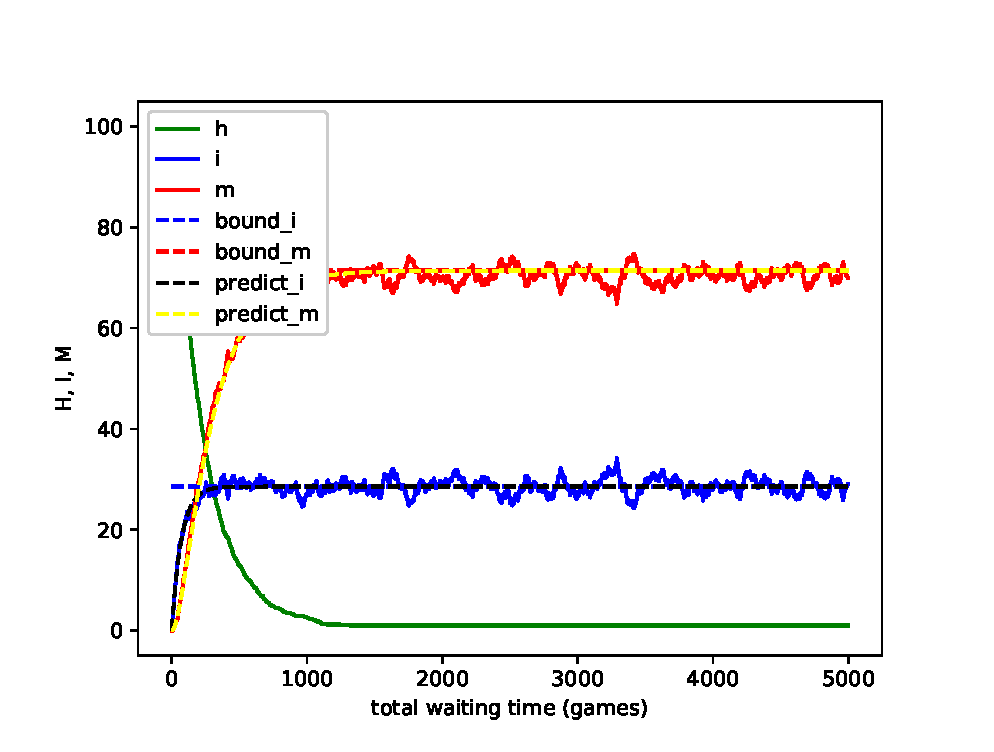
\includegraphics[width=.45\textwidth]{fig/twohop_predict_sim.eps}
  \caption{$I(t)$ and $M(t)$ with time $t$ obtained from prediction and simulations
  when $\beta = 0.004$, $\rho = 0.01$ and $N=100$. Here $h$ and $i$ is the mean value of $20$ simulations.}
  \label{fig:twohop_predict_wod}
\end{figure}
Fig.~\ref{fig:twohop_predict_wod} shows that the change of the states
in the experiments conforms to
the solved solutions.

\subsection{Optimal solution of selfish detection}
\begin{figure}
  \centering
  {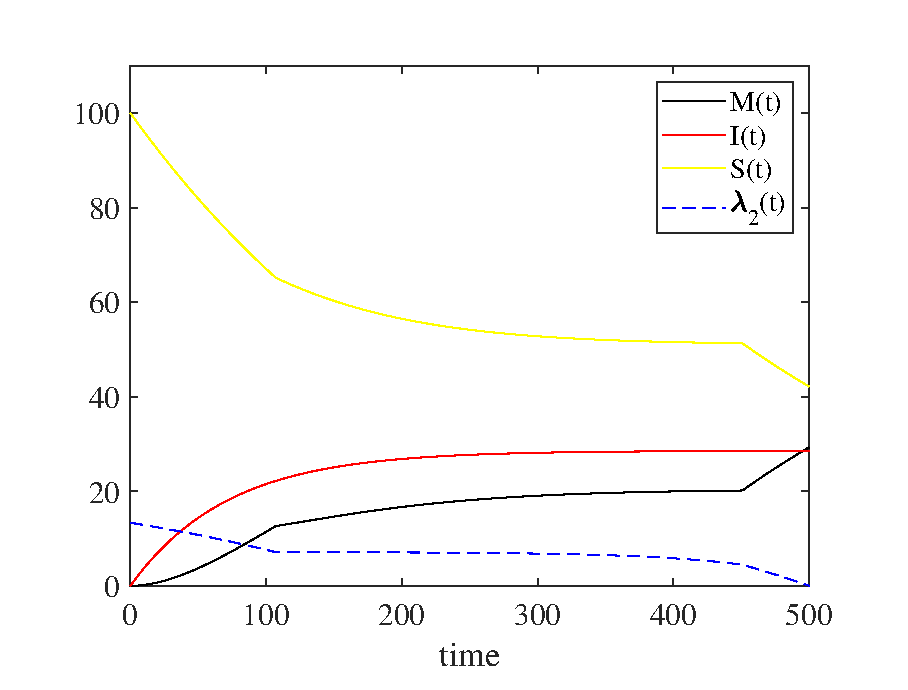
\includegraphics[width=0.47\textwidth]{fig/state.eps}}
     \caption{State variable of analysis with time.}
     \label{fig:pe_opt_state_time}
\end{figure}
\begin{figure}
  \centering
  {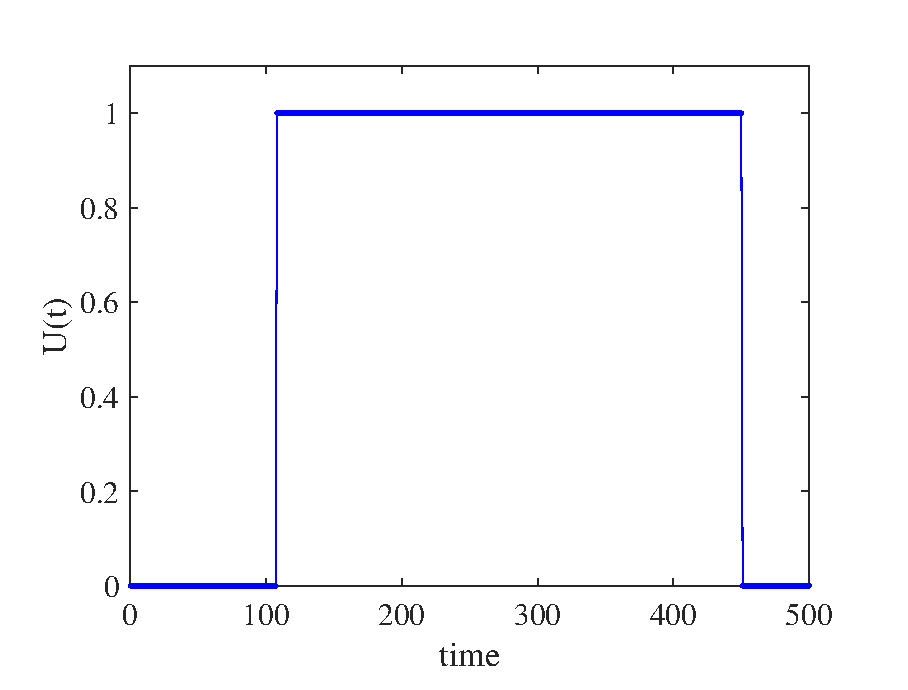
\includegraphics[width=0.47\textwidth]{fig/Ut.eps}}
     \caption{Control variable of analysis with time.}
     \label{fig:pe_opt_control_Ut}
\end{figure}
\begin{figure}
  \centering
  {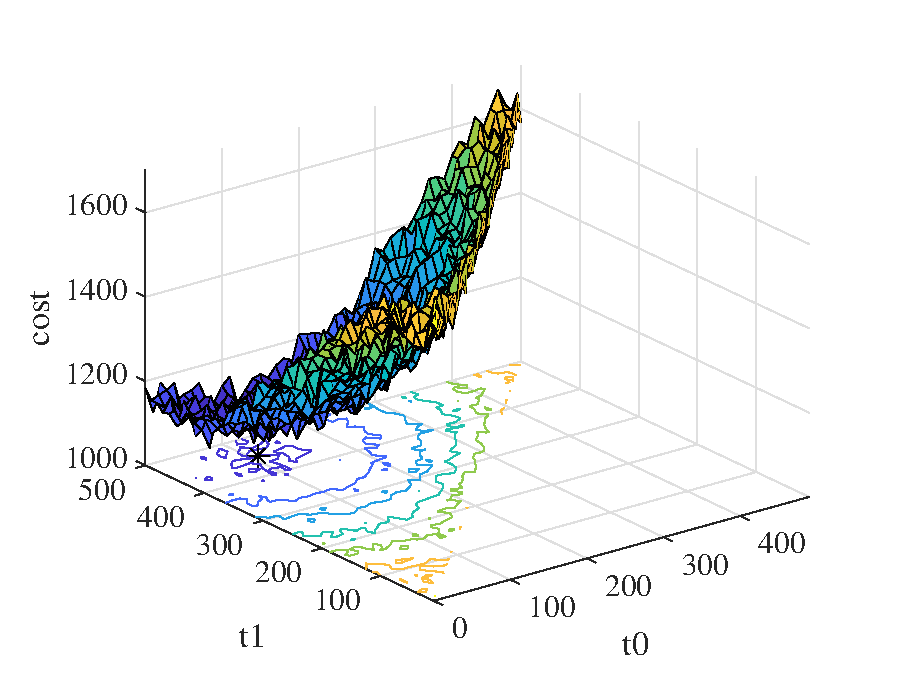
\includegraphics[width=0.47\textwidth]{fig/cost_all_t0t1.eps}}
     \caption{Different choices of $t0$ and $t1$.}
     \label{fig:pe_diff_choices}
\end{figure}

\section{Conclusion}
\label{sec:conclude}
In this paper, we have analytically investigated
the state transition of nodes in the opportunistic networks.
The ordinary differential equation models have been constructed to
capture the message dissemination with complete detection,
which can suppress the increment of selfish node number.
To achieve the tradeoff the reward and the detection cost
in the message lifetime,
we propose the optimal solution of the selfish node detection
based on the Pontryagin's maximum principle.
The soundness of the models and the accuracy of the analysis
have been verified via extensive simulation.

Through the proposed method,
it is clear that the optimal solution of selfish node detection
can be obtained
when the change rate of becoming selfish is constant.
%the strategy of the relay nodes is stable, i.e., 
%the unit paid reward is constant.
Inspired by this,
we will study effective methods 
to minimize the combination of 
the total paid reward and the detection cost
when the change rate of becoming selfish 
and the unit paid reward
are variable with time in the future.


\bibliographystyle{IEEEtran}

\bibliography{reference}

\end{document}

